\section{Bending}

Transverse loads applied to a beam causes deflections, primarily up or down is referred to as \textbf{bending}. Bending stresses depend on the beams cross-section, length, and material properties.

\subsection{Sign Conventions}

\textbf{Internal}

\begin{figure*}[!h]
\centering
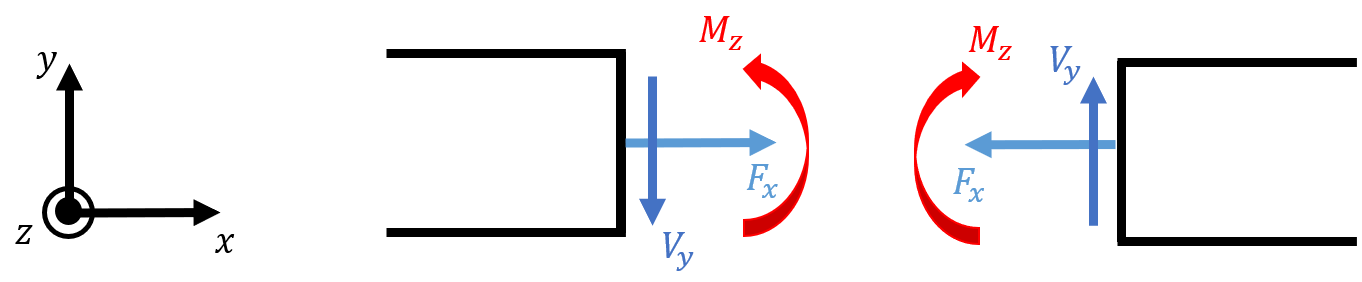
\includegraphics[angle=0, width=4in]{Bending-Figures/internalSignConvention.png}
\vspace{-2mm}
\caption{\small from reference pages}
\vspace{-3mm}
\label{Fig:InternalSigns}
\end{figure*}

\noindent \textbf{External}

\begin{figure*}[!h]
\centering
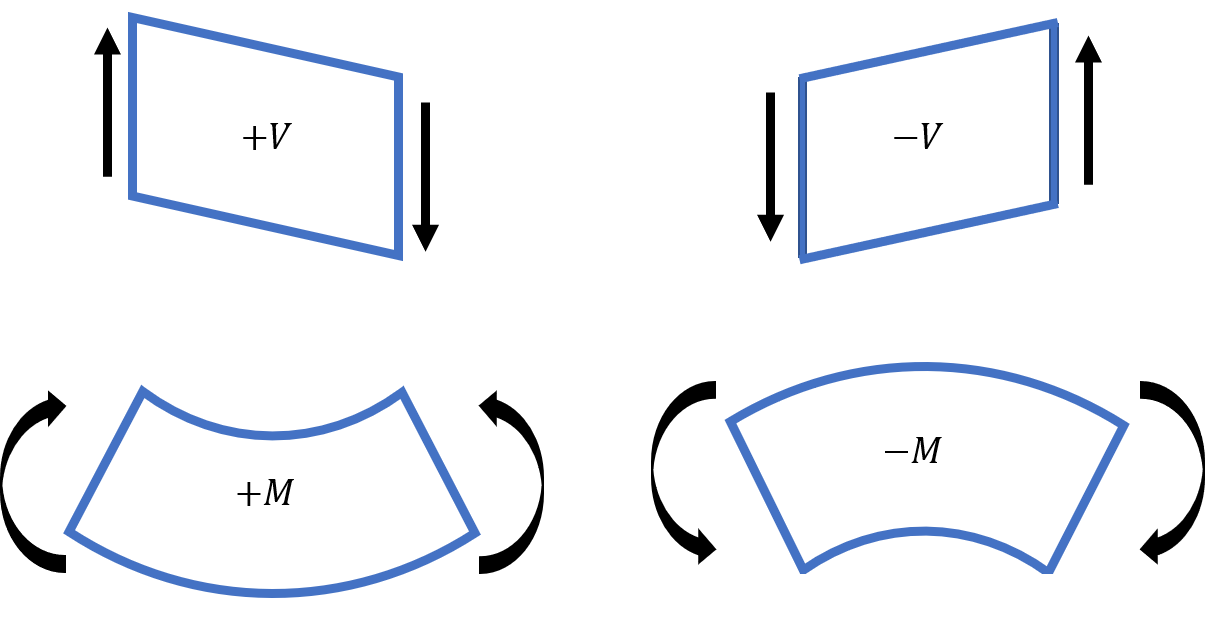
\includegraphics[angle=0, width=3.5in]{Bending-Figures/externalSignConvention.png}
\vspace{-2mm}
\caption{\small from reference pages}
\vspace{-3mm}
\label{Fig:ExternallSigns}
\end{figure*}

\subsection{Boundary Conditions}

\textbf{Statically Determinate Beams}
\begin{figure*}[!h]
\centering
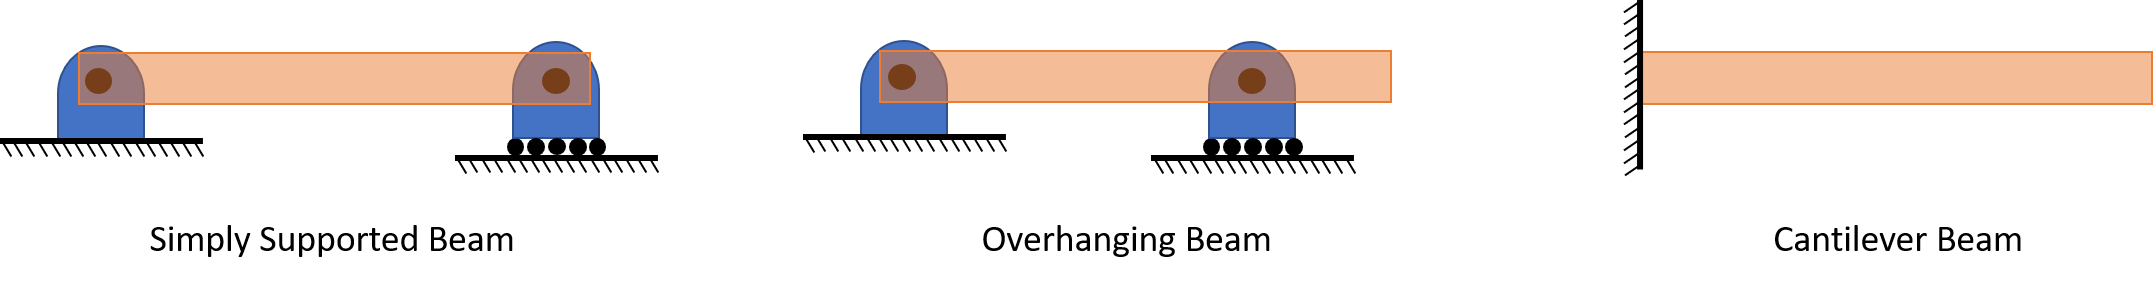
\includegraphics[angle=0, width=6in]{Bending-Figures/determinateBeams.png}
\vspace{-2mm}
\caption{\small from reference pages}
\vspace{-3mm}
\label{Fig:StaticallyDeterminate}
\end{figure*}


\noindent \textbf{Statically Indeterminate Beams}
\begin{figure*}[!h]
\centering
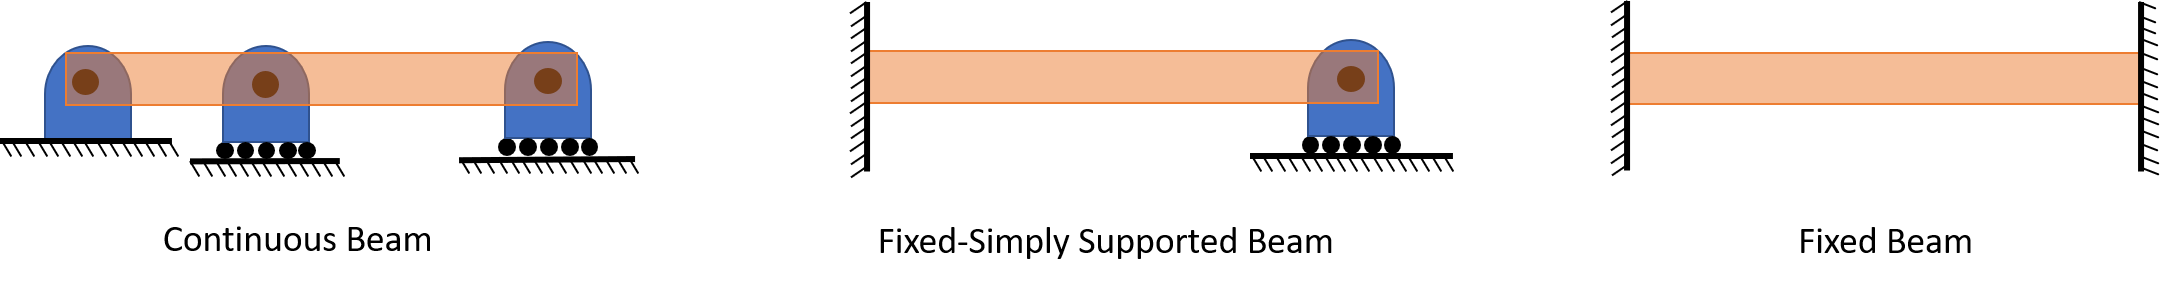
\includegraphics[angle=0, width=6in]{Bending-Figures/indeterminateBeams.png}
\vspace{-2mm}
\caption{\small from reference pages}
\vspace{-3mm}
\label{Fig:StaticallyIndeterminate}
\end{figure*}

\noindent \textbf{Loadings}
\begin{figure*}[!h]
\centering
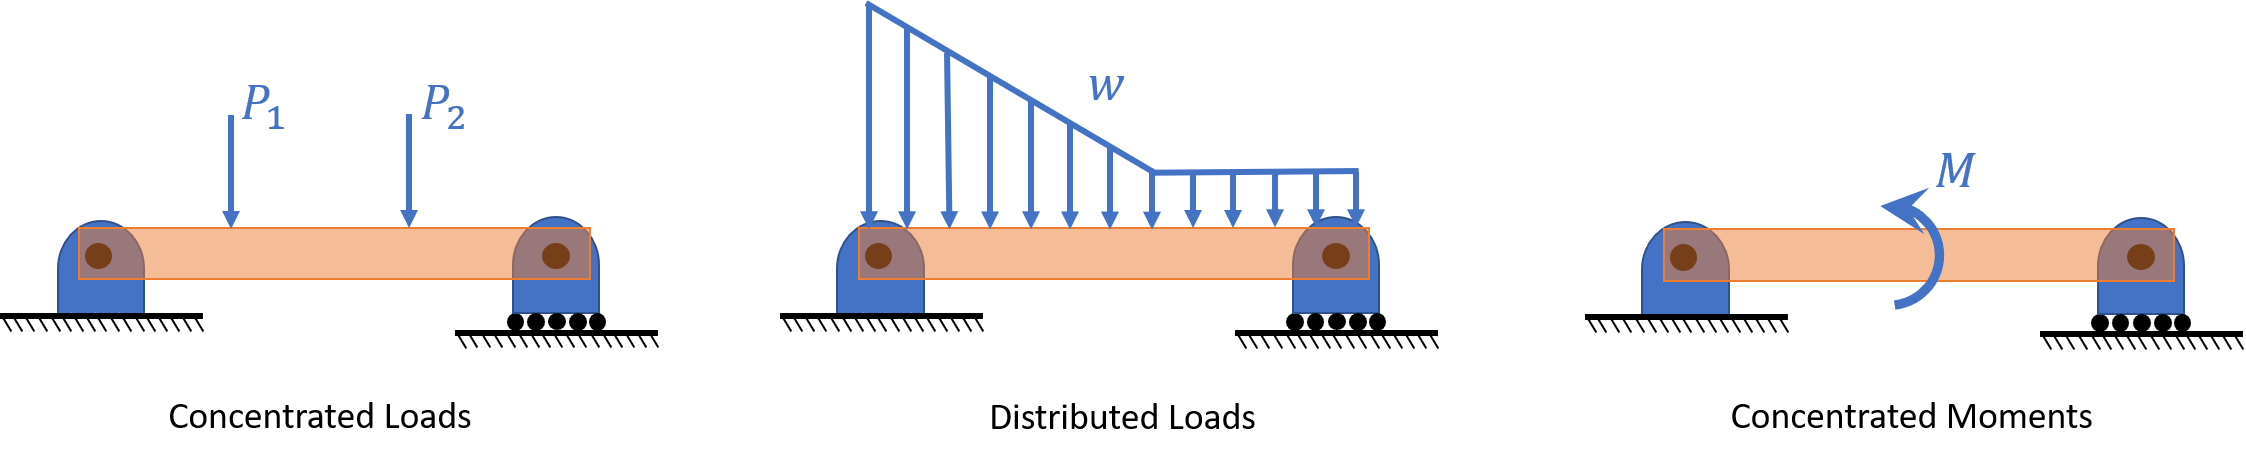
\includegraphics[angle=0, width=6in]{Bending-Figures/loadings1.png}
\vspace{-2mm}
\caption{\small from reference pages}
\vspace{-3mm}
\label{Fig:Loadings}
\end{figure*}


\subsection{\blue{Relations Among Load, Shear, and Mending Moments - does this go with Shear/Moment Diagrams?}}

\subsection{Pure Bending}

\begin{figure*}[!h]
\centering
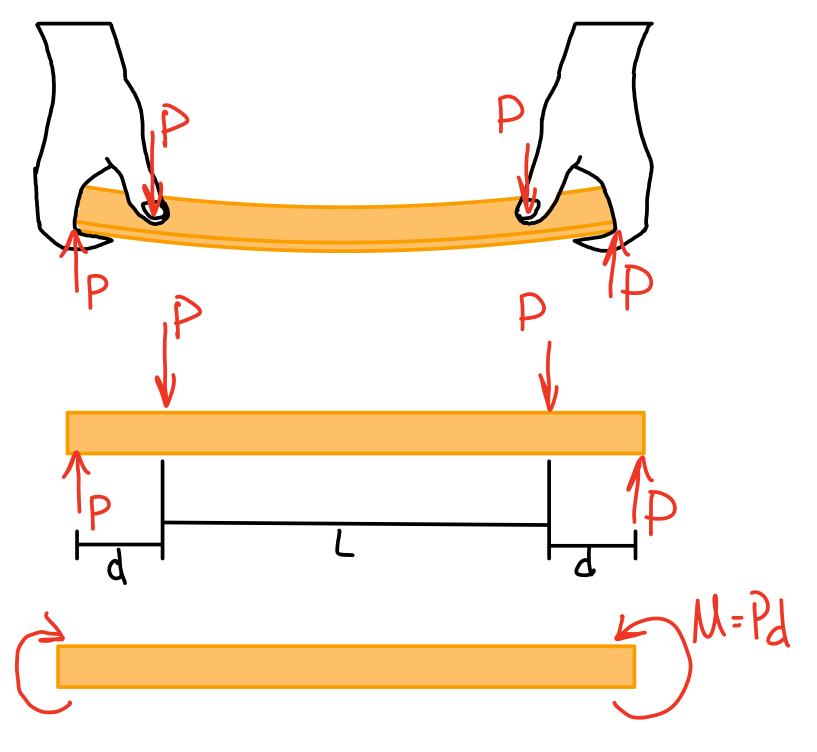
\includegraphics[angle=0, width=2in]{Bending-Figures/PureBending.png}
\vspace{-2mm}
\caption{\small \blue{Taken from TAM251 Lecture Notes - L6S11}}
\vspace{-3mm}
\label{Fig:PureBending}
\end{figure*}

Take a flexible strip, such as a thin ruler, and apply equal forces with your fingers as shown. Each hand applies a couple or moment (equal and opposite forces a distance apart). The couples of the two hands must be equal and opposite. Between the thumbs, the strip has deformed into a circular arc. For the loading shown here, just as the deformation is uniform, so the internal bending \textbf{moment is uniform}, equal to the moment applied by each hand.

\subsection{\red{Stress-Strain Variations}}

\textbf{\red{**Reference pages have a broken link image here and no text**}}

\subsection{\blue{Geometry of Deformation}}

\begin{figure*}[!h]
\centering
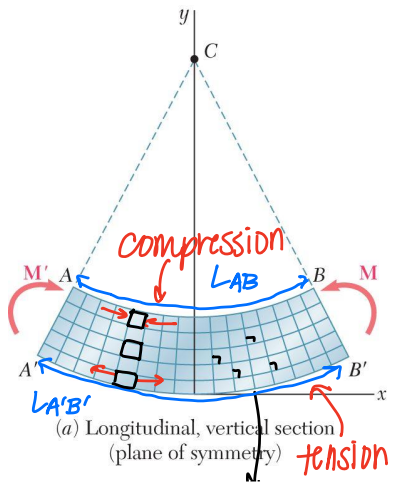
\includegraphics[angle=0, width=3in]{Bending-Figures/Geometry.png}
\vspace{-2mm}
\caption{\small \blue{Taken from TAM251 Lecture Notes - L6S12}}
\vspace{-3mm}
\label{Fig:BendingGeometry}
\end{figure*}
\blue{
\noindent Assumptions:
\begin{itemize}
    \item Plane sections remain plane $\rightarrow$ \textbf{no shear} stress/strains.
    \[\gamma_{xy} = \gamma_{xz} = 0\]
    Therefore: \[\tau_{xy} = \tau_{xz} = 0\]
    Also, traction free boundary conditions yields… \[\sigma_y = \sigma_z = \tau_{yz} = 0\]
    \item There is a \textbf{Neutral axis} between the top and the bottom where the length does not change.
    \[\sigma_x = 0 \rm\ and \rm\ \epsilon_x = 0\]
    \item The beam deforms into a \textbf{circular arc} where the top surface ($AB$) is in compression ($\sigma_x, \varepsilon_x <0$), and the bottom surface ($A'B'$) is in tension($\sigma_x, \varepsilon_x >0$).
    \item Any point in the beam is in a state of \textbf{uniaxial normal stress}.
    \item Finding stresses is a \textbf{statically indeterminate} problem.
\end{itemize}
}

\subsection{\blue{Material Behavior: linear elastic beams}}
\textbf{Elastic range:} bending moment is such that the normal stresses remain below the yield strength. Hooke’s law combined with equilibrium gives:

\noindent Defines longitudinal and neutral axes: \[\int_A y dA =0\] 
\noindent Moment-curvature equation: \[M(x) = \frac{E(x)I_z(x)}{\rho(x)}\] 

\noindent \blue{\textbf{**Expandable Derivation**}}

\noindent \blue{Constitutive Relationship:
\[L_{y_i} = L_{NAi} = L_{NAf} = \rho\theta\]
\[L_{y_f} = (\rho - y)\theta\]
\[\varepsilon_x = \frac{(\rho-y)\theta - \rho\theta}{\rho\theta}\]
\[\varepsilon_x = \frac{-y\theta}{\rho\theta} = \frac{-y}{\rho}\]
\[\sigma_x = E\varepsilon_x = -\frac{Ey}{\rho}\]}

\noindent \blue{Force Equilibrium: 
\[\Sigma F_x = 0\]
\[\Sigma F_x = \int dF\]
\[\Sigma F_x = \int \sigma_x dA\]
\[\Sigma F_x = \int\frac{-Ey}{\rho}dA\]
\[\Sigma F_x = \frac{-E}{\rho}\int y dA = 0\]}

\noindent \blue{Moment Equilibrium:
\[\Sigma M_z = -M - \int y dF = 0\]
\[\Sigma M_z = -M - \int y\sigma_x dA\]
\[\Sigma M_z = -M - \int y (\frac{-Ey}{\rho}) dA\]
\[\Sigma M_z = -M - + \frac{E}{\rho} \int y^2 dA = 0\]}

\noindent \blue{\textbf{**End Derivation**}}

\subsubsection{\blue{First Moment of Area: Centroid of an Area}}
The first moment of the area A with respect to the z-axis is given by $Q_z = \int_A y dA = \Sigma yA$ .

\vspace{5pt}

\noindent The first moment of the area A with respect to the y-axis is given by $Q_y = \int_A z dA  = \Sigma zA$.

\vspace{5pt}

\noindent \blue{The centroid of an area is at the coordinates $(\overline{x}, \overline{y})$.}

\begin{figure*}[!h]
\centering
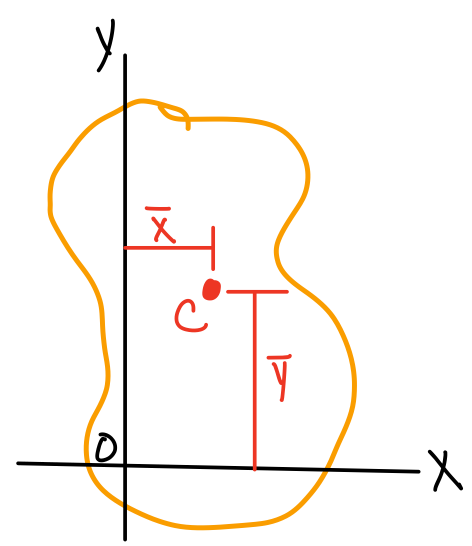
\includegraphics[angle=0, width=1in]{Bending-Figures/Centroid.png}
\vspace{-2mm}
\caption{\small \blue{Taken from TAM251 Lecture Notes - L6S19}}
\vspace{-3mm}
\label{Fig:Centroid}
\end{figure*}

\[\bar{y} = \frac{1}{A}\int_A y dA\] 
\[\bar{z} = \frac{1}{A}\int_A z dA\]

\noindent \blue{Complex (or composite) areas can be divided into smaller, easier parts.}

\begin{figure*}[!h]
\centering
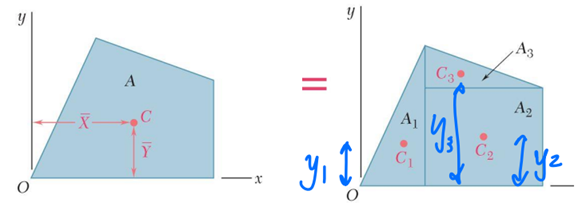
\includegraphics[angle=0, width=3.5in]{Bending-Figures/CompositeCentroid.png}
\vspace{-2mm}
\caption{\small \blue{Taken from TAM251 Lecture Notes - L6S19}}
\vspace{-3mm}
\label{Fig:CompCentroid}
\end{figure*}

\[\bar{Y} = \frac{1}{A_{tot}}\sum_i (A_i\bar{y}_i)\] \[\bar{z} = \frac{1}{A_{tot}}\sum_i (A_i\bar{z}_i)\]

\subsubsection{\blue{Second Moment or Area Moment of Inertia}}
The moment of inertia of the area A with respect to the z-axis is given by $I_z = \int_A y^2 dA$.

\vspace{5pt}

\noindent The moment of inertia of the area A with respect to the y-axis is given by $I_y = \int_A z^2 dA$.

\vspace{5pt}

\noindent \textit{Note:}  polar moment of inertia in this plane \[J = \int_A \rho^2 dA = \int_A (y^2 + z^2)dA = I_y + I_z\]

\begin{figure*}[!h]
\centering
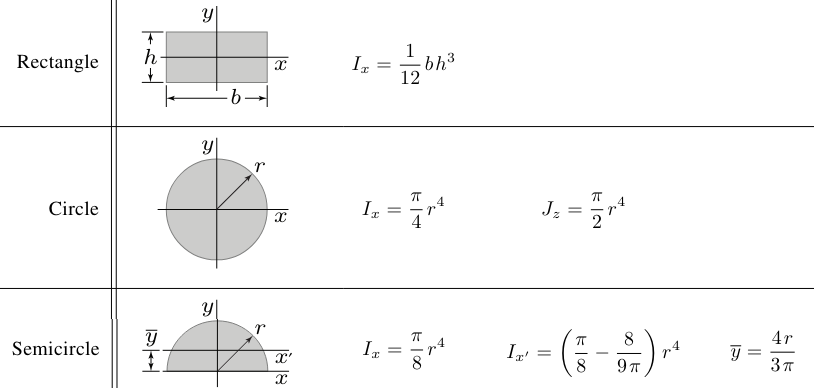
\includegraphics[angle=0, width=3.5in]{Bending-Figures/CommonShapes.png}
\vspace{-2mm}
\caption{\small \blue{From the formula sheet}}
\vspace{-3mm}
\label{Fig:Common Shapes}
\end{figure*}

\noindent \textbf{Parallel-axis theorem:} the moment of inertia about an axis through C’ parallel to the axis through the centroid C is related to $I_C$ by \[I_C = I_{C'} +A'd_{CC'}^2\]

\subsubsection{\blue{Maximum Normal Stress}}
From equilibrium: the centroid is located at $\bar{y}=0$, i.e., \textit{the neutral axis passes through the centroid of the section}.

\vspace{5pt}

\noindent Elastic Flextural Formula \[\sigma_x (x,y) = - \frac{M(x)y}{I_z(x)}\]

\noindent \blue{\textbf{**Expandable Derivation**}}

\blue{
\[M_z = \frac{EI_z}{\rho}\]
\[M_z = \frac{-\sigma_x}{y}I_z\]
}
\noindent \blue{\textbf{**End Derivation**}}

\noindent To evaluate the maximum absolute normal stress, denoting “c” the largest distance from the neutral surface, we use:

\begin{figure*}[!h]
\centering
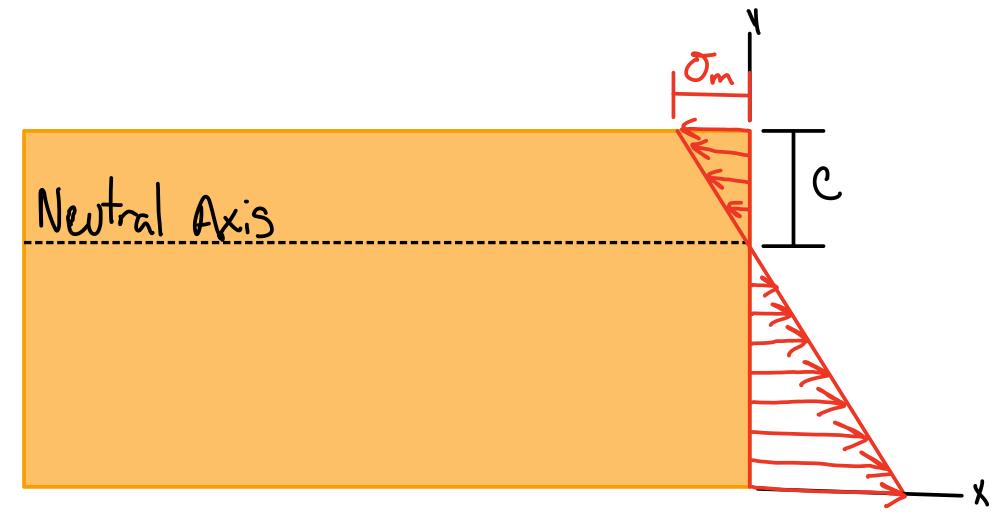
\includegraphics[angle=0, width=2in]{Bending-Figures/MaxStress.png}
\vspace{-2mm}
\caption{\small \blue{Taken from TAM251 Lecture Notes - L6S17}}
\vspace{-3mm}
\label{Fig:MaxStress}
\end{figure*}

\[\sigma_{max} = \frac{|M|c}{I_z}\]

\noindent Note that the ratio I/c depends only upon the geometry of the cross section. This ratio is called the ELASTIC SECTION MODULUS and is denoted by S:

\[\sigma_{max} = \frac{|M|}{S}\]
Where \[S = \frac{I}{c}\]

\subsection{Composite Beams \cyan{BSM: no longer covered in TAM 251, not sure if/when it is covered in ME curriculum.}}

Recall that $\epsilon_x = -\frac{y}{\rho}$ does not depend on the material properties of the beam, and is based only on the assumptions of geometry done so far.

\vspace{5pt}

\noindent \textbf{\red{**Reference pages have a broken link image here**}}

\vspace{5pt}

\noindent In non-homogeneous beams, we can no longer assume that the neutral axis passes through the centroid of the composite section. We should now determine that location…

\vspace{5pt}

\noindent After obtaining the TRANSFORMED CROSS SECTION, we get
\[\int_{A_t}y d A_t = 0\]

\noindent Therefore, the neutral axis passes through the centroid of the transformed cross section.

\noindent Note that the widening ($n > 1$) or narrowing ($n < 1$) must be done in a direction parallel to the neutral axis of the section, since we want y-distances to be the same in the original and transformed section, so that the distance y in the flexural formula is unaltered.

\[\sigma_1 = -\frac{My}{I_t}\]
\[\sigma_2 = -\frac{nMy}{I_t}\]


\subsection{Eccentric Axial Loading in a Plane of Symmetry}

Equilibrium gives:\[F=P \ \ \text{and} \ \ M=Pd\]

\noindent \textbf{\red{**Reference pages have a broken link image here**}}

\vspace{5pt}

\noindent Stress due to eccentric loading found by superposing the uniform stress due to a centric load and linear stress distribution due to a pure bending moment.

\vspace{5pt}

\noindent \textbf{\red{**Reference pages have a broken link image here**}}

\vspace{5pt}

\noindent Validity requires stresses below proportional limit (elastic region), deformations have negligible effect on geometry, and stresses not evaluated near points of load application.





